\documentclass[letterpaper]{article}
\usepackage[utf8]{inputenc}
\usepackage{pgf, tikz}
\usepackage{pgfplots}
\usetikzlibrary{arrows, automata}
\usetikzlibrary{graphs, graphs.standard}
\usepackage{amsmath}
\tikzset{
  common/.style={draw,name=#1,node contents={},inner sep=0,minimum size=3},
  disc/.style={circle,common=#1},
  square/.style={rectangle,common={#1}},
}

\begin{document}

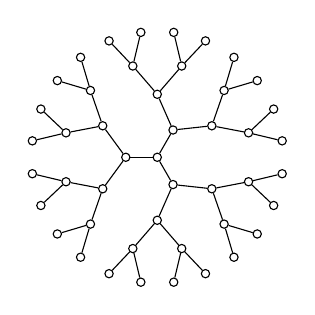
\begin{tikzpicture}[scale = 0.4]
  \draw (0,0) node[disc=c-0-1];
  \xdef\radius{0cm}
  \xdef\level{0}
  \xdef\nbnodes{1}
  \xdef\degree{(3+1)} % special degree just for the root node
  \foreach \ndegree/\form in {3/disc,3/disc,3/disc,3/disc}{
    \pgfmathsetmacro\nlevel{int(\level+1)}
    \pgfmathsetmacro\nnbnodes{int(\nbnodes*(\degree-1))}
    \pgfmathsetmacro\nradius{\radius+1cm}
    \draw[white] (c-0-1) circle(\nradius pt);
    \foreach \div in {1,...,\nnbnodes} {
      \pgfmathtruncatemacro\src{((\div+\degree-2)/(\degree-1))}
      \path (c-0-1) ++({\div*(360/\nnbnodes)-180/\nnbnodes}:\nradius pt) node[\form=c-\nlevel-\div];
      \draw (c-\level-\src) -- (c-\nlevel-\div);
    }
    \xdef\radius{\nradius}
    \xdef\level{\nlevel}
    \xdef\nbnodes{\nnbnodes}
    \xdef\degree{\ndegree}
  }
\end{tikzpicture}

\end{document}